%%%%%%%%%%%%%%%%%%%%%%%%%%%%%%%%%%%%%%%%%%%%%%%%%%%%%%%%%%%%%%%%%%%%%%
% How to use writeLaTeX: 
%
% You edit the source code here on the left, and the preview on the
% right shows you the result within a few seconds.
%
% Bookmark this page and share the URL with your co-authors. They can
% edit at the same time!
%
% You can upload figures, bibliographies, custom classes and
% styles using the files menu.
%
% If you're new to LaTeX, the wikibook is a great place to start:
% http://en.wikibooks.org/wiki/LaTeX
%
%%%%%%%%%%%%%%%%%%%%%%%%%%%%%%%%%%%%%%%%%%%%%%%%%%%%%%%%%%%%%%%%%%%%%%
\documentclass{tufte-handout}

%\geometry{showframe}% for debugging purposes -- displays the margins

\usepackage{amsmath}

% Set up the images/graphics package
\usepackage{graphicx}
\setkeys{Gin}{width=\linewidth,totalheight=\textheight,keepaspectratio}
\graphicspath{{graphics/}}

\title{Presenting Data and Information: A Summary of the Edward Tufte Course and Its Relevant Lessons for NCAR Scientists}
\author[David John Gagne]{David John Gagne II}
\date{25 July 2017}  % if the \date{} command is left out, the current date will be used

% The following package makes prettier tables.  We're all about the bling!
\usepackage{booktabs}

% The units package provides nice, non-stacked fractions and better spacing
% for units.
\usepackage{units}

% The fancyvrb package lets us customize the formatting of verbatim
% environments.  We use a slightly smaller font.
\usepackage{fancyvrb}
\fvset{fontsize=\normalsize}

% Small sections of multiple columns
\usepackage{multicol}

% Provides paragraphs of dummy text
\usepackage{lipsum}
\usepackage{url}
% These commands are used to pretty-print LaTeX commands
\newcommand{\doccmd}[1]{\texttt{\textbackslash#1}}% command name -- adds backslash automatically
\newcommand{\docopt}[1]{\ensuremath{\langle}\textrm{\textit{#1}}\ensuremath{\rangle}}% optional command argument
\newcommand{\docarg}[1]{\textrm{\textit{#1}}}% (required) command argument
\newenvironment{docspec}{\begin{quote}\noindent}{\end{quote}}% command specification environment
\newcommand{\docenv}[1]{\textsf{#1}}% environment name
\newcommand{\docpkg}[1]{\texttt{#1}}% package name
\newcommand{\doccls}[1]{\texttt{#1}}% document class name
\newcommand{\docclsopt}[1]{\texttt{#1}}% document class option name

\begin{document}

\maketitle% this prints the handout title, author, and date

\begin{abstract}
\noindent I recently attended the one-day course on ``Presenting Data and Information" by Edward Tufte, a major pioneer of data visualization, thanks to generous support from Dr. Doug Nychka and IMAGe. During the course, Tufte covered important principles of analytical design and guidelines for giving effective presentations. He also provided his perspective on a wide range of topics related to data visualization and showcased visualizations that exemplified his design principles. In this seminar, I will highlight important lessons from the course, analyze some of the featured visualizations, and discuss how NCAR scientists can incorporate these design principles into their scientific workflows.
\end{abstract}

Edward Tufte is a professor emeritus of political science, statistics, and computer science at Yale University. He is a pioneer in the field of data visualization and information design and has written four books on the subject: \textit{The Visual Display of Quantitative Information}, \textit{Envisioning Information}, \textit{Visual Explanations}, and \textit{Beautiful Evidence}. In his books, he discusses many examples of effective and defective visualizations and how design choices can either illuminate or obscure the information being presented. Through his course, Tufte explains his views on data visualization.

\begin{figure}
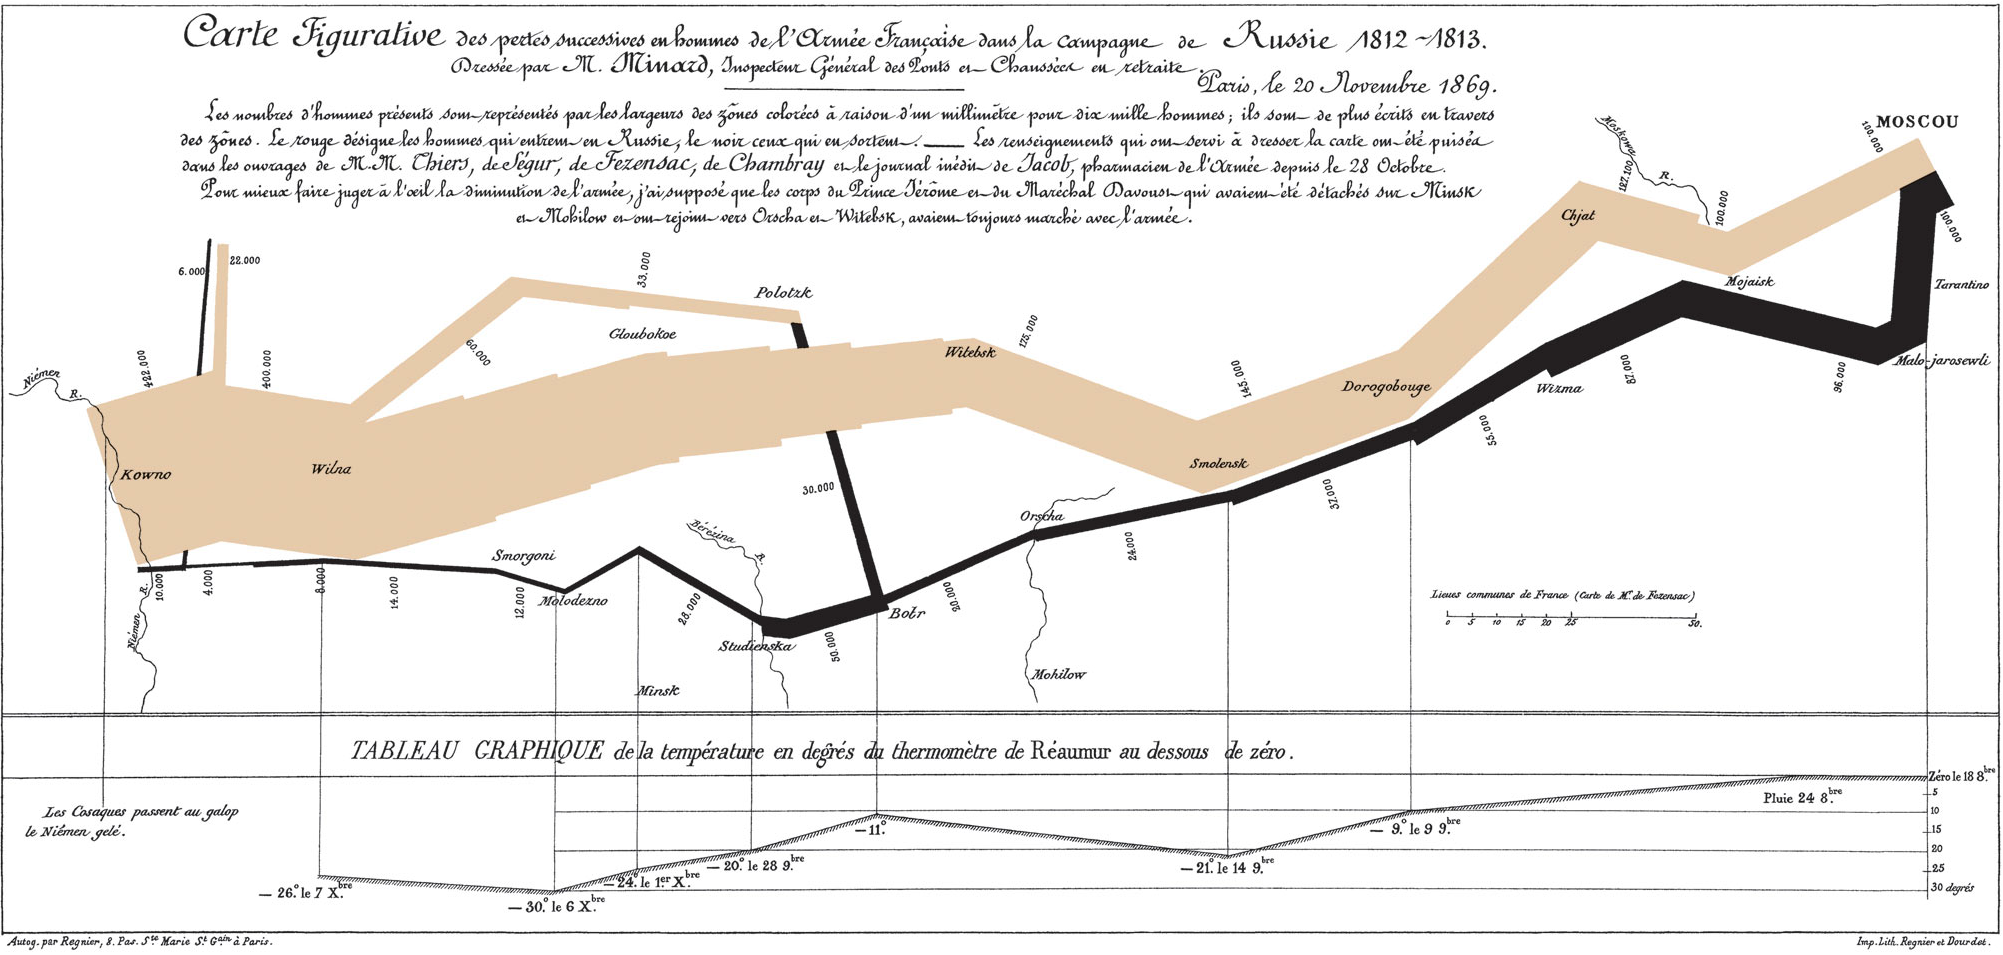
\includegraphics[width=\textwidth]{Minard.png}
\caption{A map of the French Army's march through Russia in the winter of 1812-1813 by Charles Joseph Minard.}
\end{figure}

\section{Principles of Analytical Design}
Charles Joseph Minard's data map of the march of Napoleon's army to Moscow and back exemplifies all of the fundamental principles of analytical design\footnote{For a full discussion of these principles, read Tufte, E., \textit{Beautiful Evidence}, pages 122-139.}. The first principle is to \textit{show comparisons, contrasts, and differences}. The Minard map compares the size of the Army through time with the width of the line and annotations of the Army size at different times. The second principle is to \textit{show causality, mechanism, explanation, and systematic structure}. The Minard map links the deaths on the retreat to a series of cold temperatures along the route.

The third principle is to \textit{show multivariate data}, which in the Minard map can be seen with six dimensions of information clearly laid out on one image. The fourth principle recommends \textit{completely integrating words, numbers, images, and diagrams}. In his graphic, Minard includes text describing the chart, the path of the Army, annotations of the number of soldiers at different points, rivers, and both a time series and text representations of the temperature. These are combined together on the same image to use as many modes of evidence as possible to do everything it takes to explain something. 

The fifth principle is to \textit{thoroughly describe the evidence. Provide a detailed title, indicate the authors and sponsors, document the data sources, show complete measurement scales, and point out relevant issues}. Minard documents all of his sources of information, his assumptions, and provides measurement scales for all data in order to bolster the credibility of the graphic. The final principle is that \textit{analytical presentations ultimately stand or fall depending on the quality, relevance, and integrity of their content}. Minard's graphic is powerful because of the underlying narrative about the horrors of war expressed through the depiction of the march. The most effective way to improve a presentation is to get better content.

\section{Effective Presentations}
Tufte wants us to present our evidence more effectively so that our audiences are better informed and can make wiser decisions. Unfortunately, the prevalence of PowerPoint slide presentations and the cognitive framework induced by them has led to shallower analysis and the obfuscation of important or inconvenient evidence under a pile of bullet points. The frequent use of slides, as opposed to narrative documents like memos or technical reports, contributed to the decisions that doomed both the Challenger and Columbia space shuttles\footnote{The Columbia investigation is described in \textit{Beautiful Evidence}, pages 162-168; the Challenger accident is covered in \textit{Visual Explanations}, pages 38-52.}. The key issues are that slides break information into separate chunks in time, slides are a far lower resolution medium than paper and even speech, and bullet points enforce a false hierarchy of information often disconnected from causality or the true narrative of the evidence.

To break free from the shackles of PowerPoint, Tufte recommends using narrative documents as the primary medium for the meeting, or in short, use Word instead of PowerPoint. The presenter should arrive early as a precaution against technical and logistical difficulties and as a sign of respect to the audience. At the beginning of the meeting, the presenter should distribute a narrative handout with relevant graphics approximately 4 pages in length. The audience should spend the first 5-10 minutes of the meeting reading the document. Then, the presenter guides the audience through the document and moderates any resulting discussions. PowerPoint can still be used to display graphics and videos. Any visualizations should be created with the principles of analytical design in mind and should not be dumbed down. Having endless respect and optimism about the audience is key and will show through your presentation style. Finally, the presenter should finish early because it respects the audience's time. 
\section{Relevant Lessons for NCAR Scientists}
In addition to the broader themes of analytical design and effective presentations, Tufte offered commentary and advice on a wide range of issues related to information visualization. When constructing visualizations on lower resolution displays, spatial scrolling instead of temporal stacking is the preferred way to layer information. Slow panning of images can provide the illusion of depth while conveying more spatial information in a given time frame. Direct annotation of points on a plot conveys meaning more quickly and directly than decoding through a legend. Simple tables of numbers can convey more information than a stack of bar, pie, and line charts. Mixing text and graphics creates far more effective visuals than using either in isolation\footnote{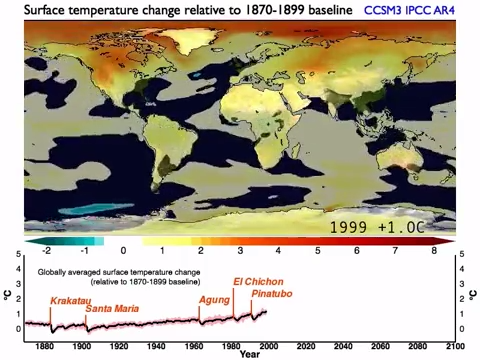
\includegraphics[width=2.5in]{ccsm_video.png} NCAR CCSM climate change simulation visualization.}. 

What tools should be used to create data visualization and documentation? Tufte recommended Python, R, D3.js, and \LaTeX ~for high-end work and Adobe Illustrator for finishing publication-quality graphics. As a visualization and documentation medium, the Jupyter Notebook package, in my opinion, adheres very closely to Tufte's principles of analytical design and recommendations for effective presentations. Jupyter Notebooks consist of cells of either software code, text, or graphics arranged vertically. Users can input plain text, HTML, or \LaTeX ~into the text cells so that explanations, links, and equations are grouped together. The software cells link with kernels for many popular data analysis languages, including Python, R, and Julia; and the graphics are generated and displayed inline with the document. Notebooks can be viewed natively in the browser, export to pdf, or rendered on Github.

One key strategy for building better visualizations is finding quality examples that convey similar kinds of information to one's own and emulating their design principles. Tufte recommends emulating visuals in your field that are successful in the wild. For general visualization, Tufte recommended Google Maps, the New York Times, ESPN, and xkcd. Figures in \textit{Science} and \textit{Nature} often have to compress a lot of information into a small area and receive many views, so they are another area to look for ideas. NCAR also has many experts in data visualization, and they have produced many exemplary visualizations that follow the analytical design principles. With the trend toward open source programming and open science, more science visualizations and their source code are now publicly available. For example, the LIGO gravitational wave detection group has published Jupyter Notebooks displaying their full analysis procedure for each event. Also, the \textit{Python Data Science Handbook} is available as a repository of Jupyter Notebooks for each section of the book. 

To conclude, I want you to consider your current scientific visualization and preparation framework. What tools and techniques have helped you create effective visualizations and presentations? What challenges do you continue to face when building and communicating visual scientific data? Where do you need to improve your visualization and presentation techniques the most?  

\section{Visualization Examples}
\begin{enumerate}
\item National Weather Service Forecast Page\footnote{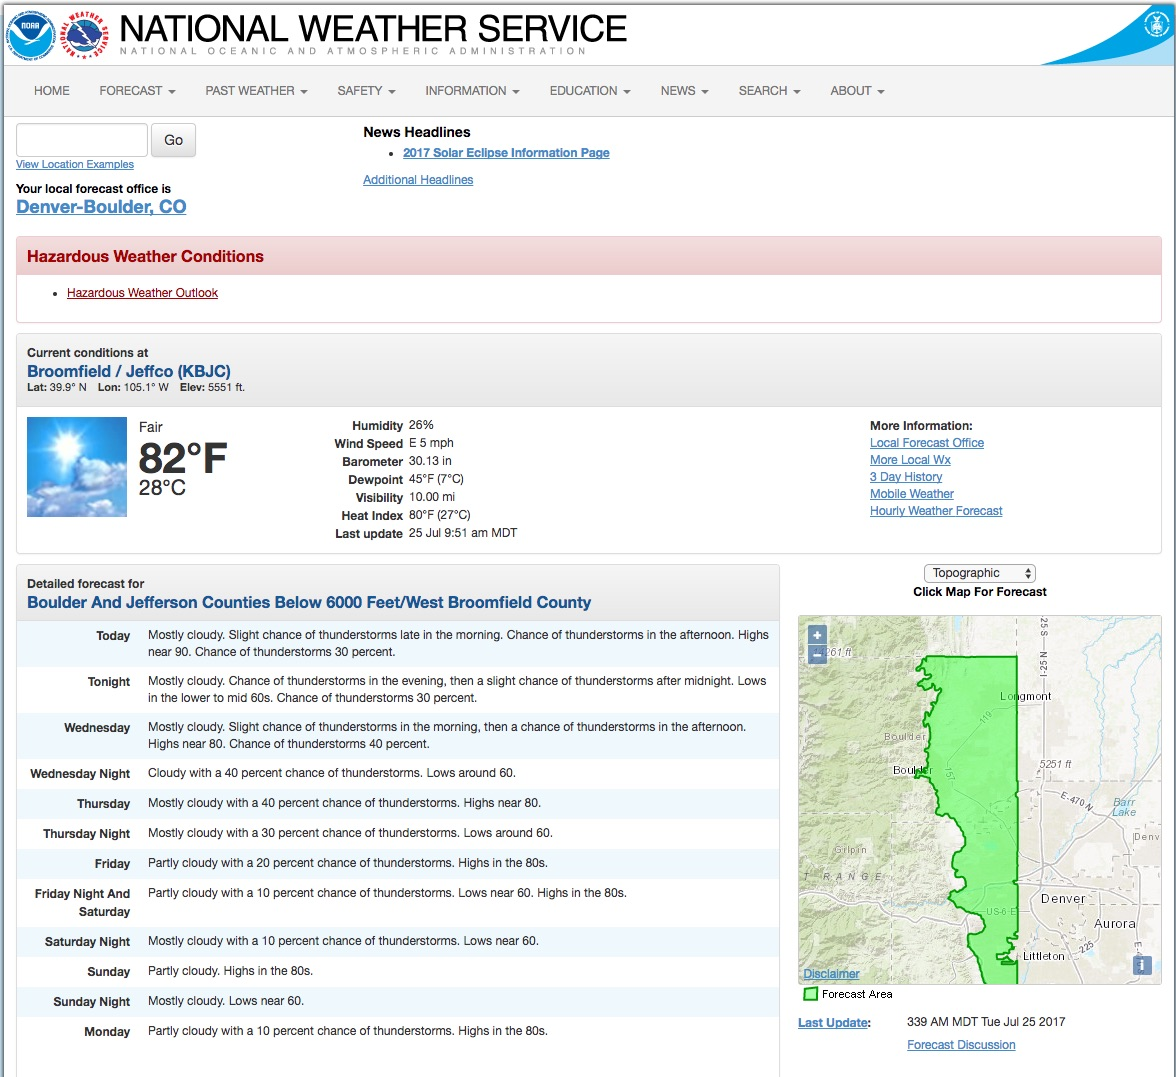
\includegraphics[width=2in]{nws_page.jpg} National Weather Service forecast page.}: \url{http://forecast.weather.gov/MapClick.php?lat=40.01574000000005&lon=-105.27923999999996
}
\item{Stephen Malinowski's Music Animation Machine\footnote{
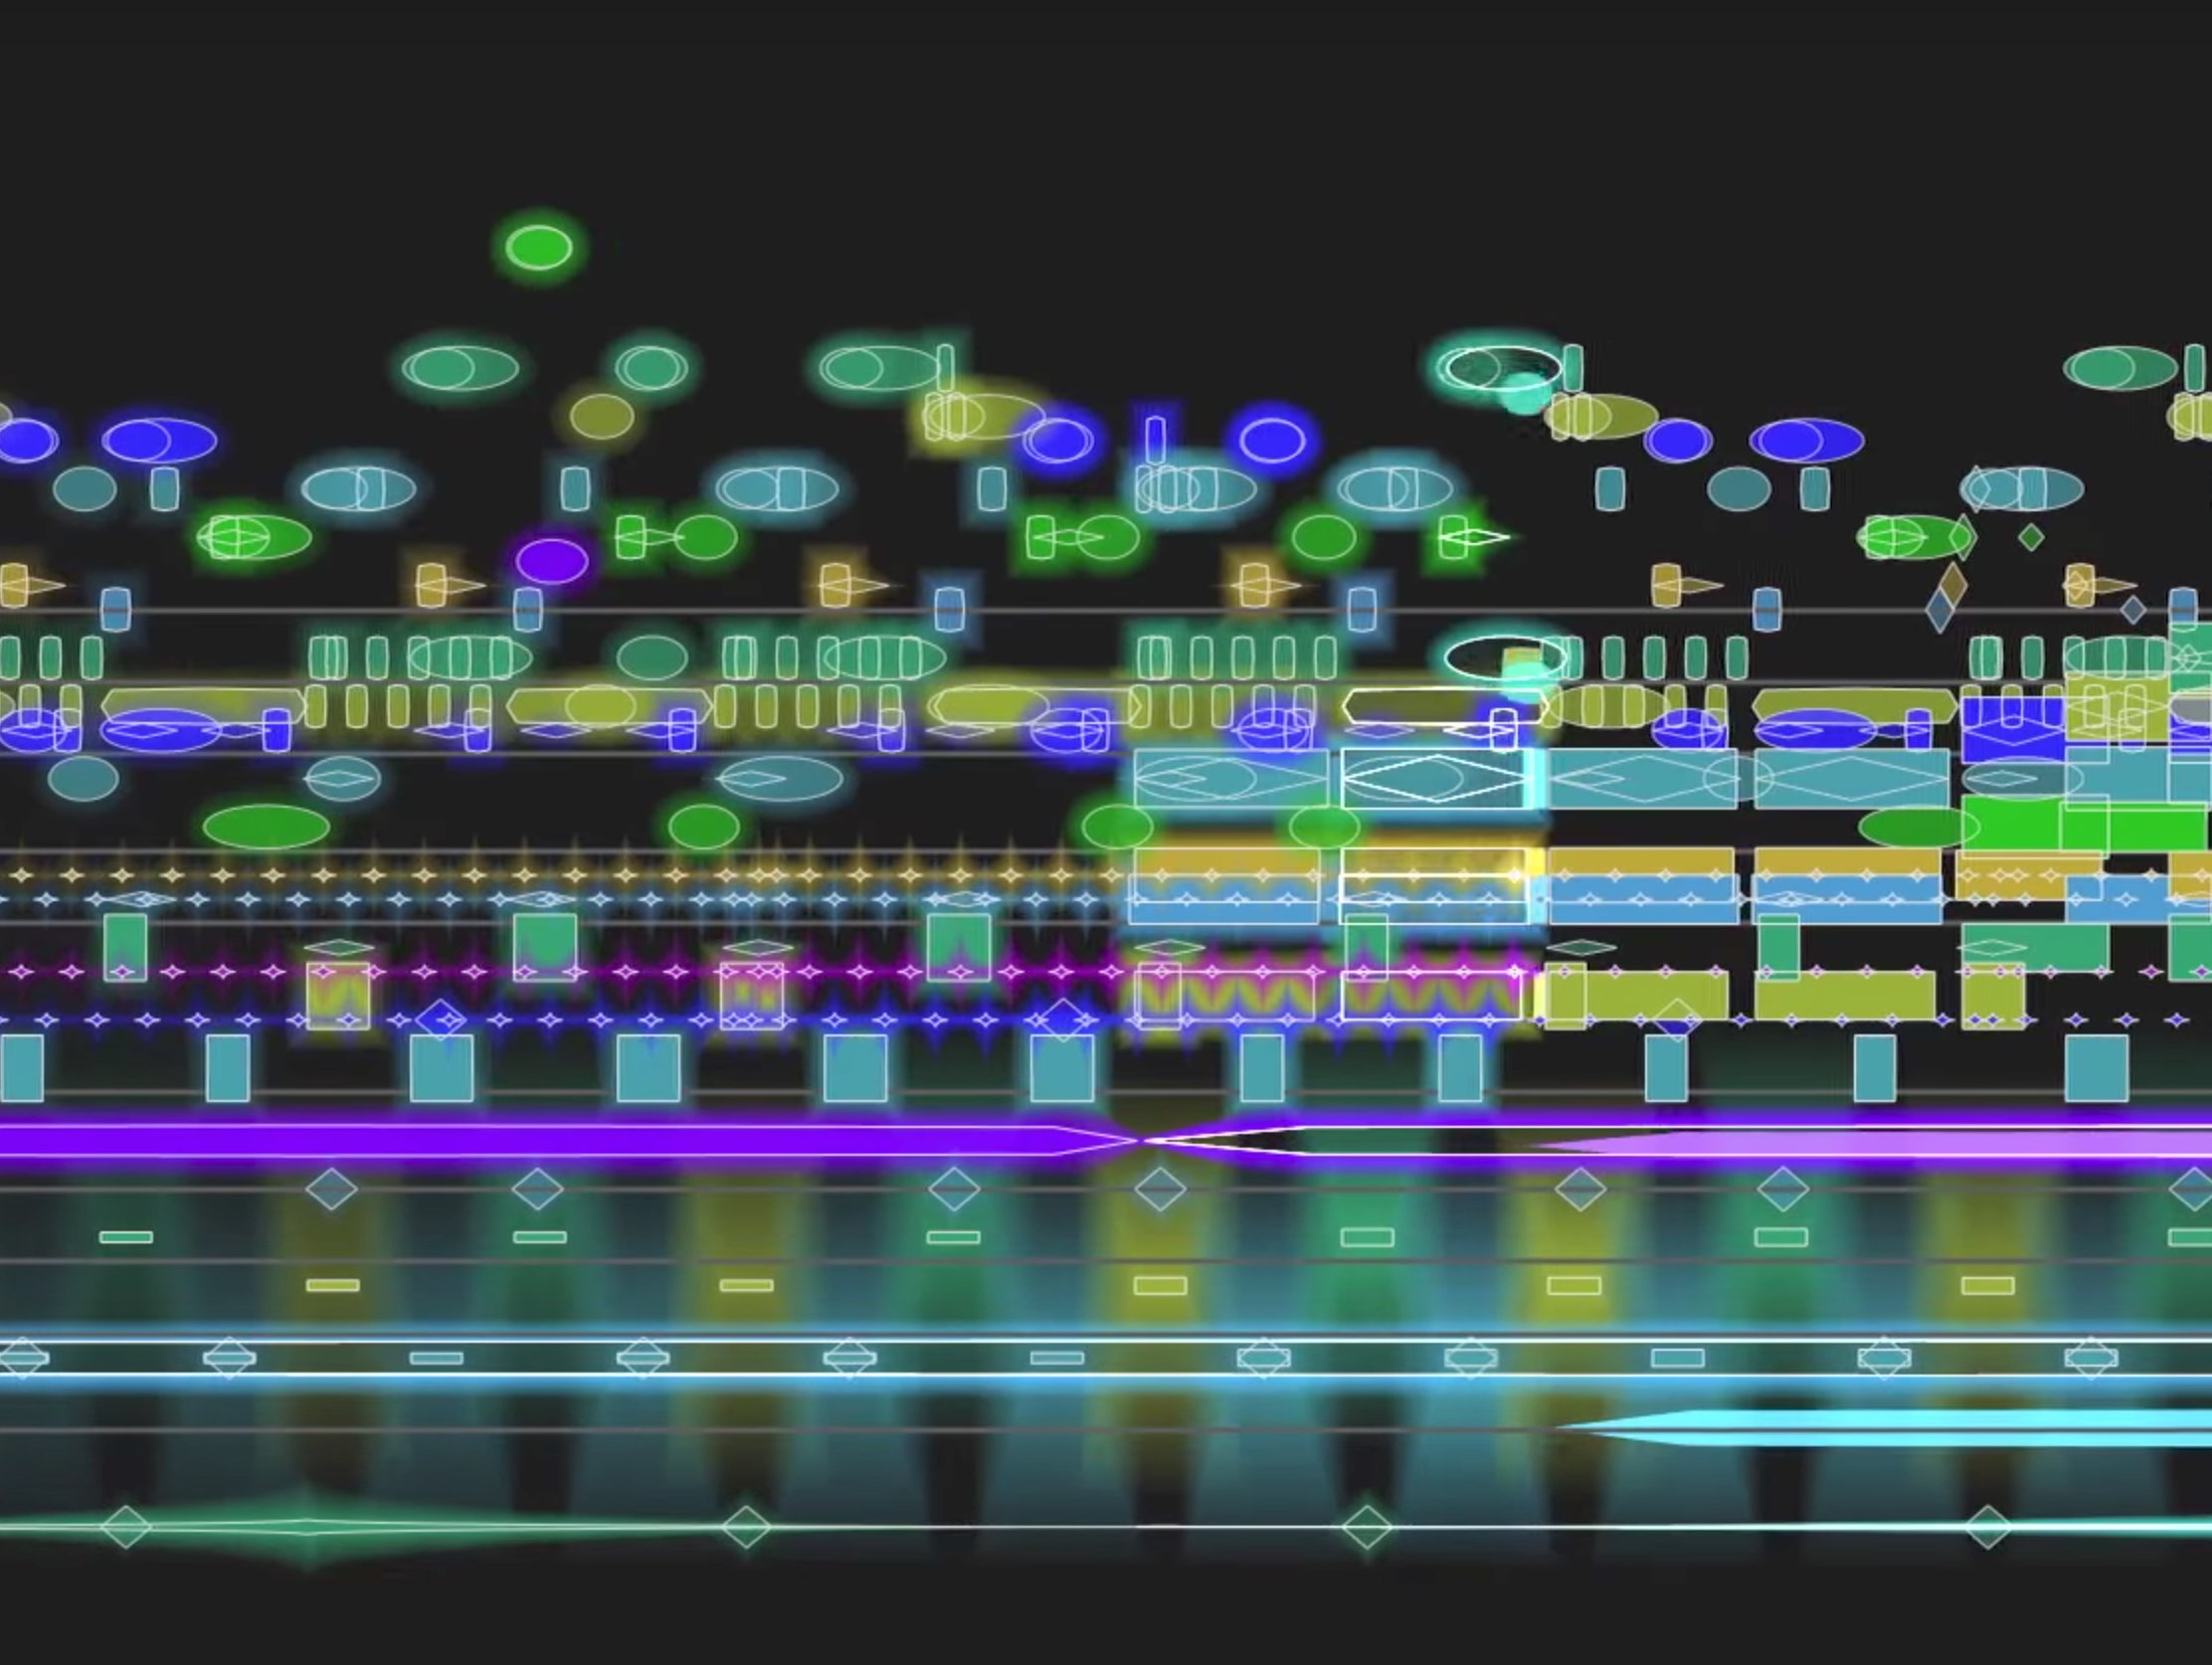
\includegraphics[width=2in]{rite_of_spring.jpg}
Music Animation Machine depiction of Igor Stravinsky's \textit{The Rite of Spring}.}: \url{https://musanim.com/watch_mam.html}}
\item{NCAR CCSM Climate Change Video: \url{https://www.vets.ucar.edu/vg/IPCC_CCSM3/index.shtml}}
\item{LIGO Open Science Center: \url{https://losc.ligo.org/tutorials/}}
\item{Python Data Science Handbook: \url{https://github.com/jakevdp/PythonDataScienceHandbook}}
\item{NCAR Ensemble Sounding Viewer: \url{http://ensemble.ucar.edu/sounding.php?d=2017072400}}
\end{enumerate}

\end{document}